\documentclass[12pt]{article}

\usepackage[russian]{babel}
\usepackage{hhline}
\usepackage{graphicx}

\graphicspath{{pictures/}}
\DeclareGraphicsExtensions{.png}
\usepackage{multirow}
\usepackage{amsmath}
\usepackage{mathtext}
\usepackage[T2A]{fontenc}
\usepackage[utf8]{inputenc}
\usepackage{pscyr} 
\usepackage[left=1cm,right=1.5cm, top=1cm,bottom=1cm,bindingoffset=0cm]{geometry}
\begin{document}

\pagestyle{empty}
\begin{center}
\large{\textbf{Университет ИТМО}}
\end{center}
\rule{550pt}{1pt}
\par\bigskip\par\bigskip\par\bigskip\par\bigskip\par\bigskip\par\bigskip\par\bigskip\par\bigskip
\begin{center}
\Large
\textbf{Отчёт по лабораторной работа №3}

\textbf{\textit{«Исследование характеристик источника тока»}}


\end{center}
\par\bigskip\par\bigskip\par\bigskip\par\bigskip\par\bigskip\par\bigskip\par\bigskip\par\bigskip\par\bigskip\par\bigskip\par\bigskip\par\bigskip\par\bigskip\par\bigskip      
\begin{flushright}
\large
Выполнил: Федюкович С. А.
\par\bigskip
Факультет: МТУ “Академия ЛИМТУ”
\par\bigskip
Группа: S3100                       
\par\bigskip\par\bigskip\par\bigskip

\rule{150pt}{0.5pt}
\par\bigskip\par\bigskip\par\bigskip\par\bigskip                                                            
 Проверил: Пшеничнов В. Е.
\par\bigskip \par\bigskip

\rule{150pt}{0.5pt}
\end{flushright}
\par\bigskip\par\bigskip\par\bigskip\par\bigskip\par\bigskip\par\bigskip\par\bigskip\par\bigskip\par\bigskip\par\bigskip     
\begin{center}
\large
Санкт-Петербург
\par\bigskip
2018
\end{center}
\newpage
\section*{Цель работы}
Исследовать зависимость полной мощности, полезной мощности, мощности потерь, падения напряжения во внешеней цепи и КПД источника от силы тока в цепи. 
\section*{Краткое теоретическое описание}
Если к источнику тока, обладающим внутренним сопротивлением $r$ подключить внешнее сопротивление $R$, то напряжение на зажимах источника $U$, согласно закону Ома для неоднородного учатска цеи можно представить в виде:
\begin{equation}
U = \varepsilon -Ir,
\end{equation}
где $\varepsilon$ --- электродвижущая сила источника (ЭДС); $I$ --- сила тока, текущего через источник.

Из уравнения (1) получаем следующее: 
\begin{equation}
I\varepsilon=I^2R + I^2R,
\end{equation}
которое можно представить в виде:
\begin{equation}
P=P_1+P_2.
\end{equation}
Здесь $P=I\varepsilon$ --- полная мощность, развиваемая источником; $P_1 = IU$ --- полезная мощность; $P_2 = I^2r$ --- потери мощности во внутри источника (на сопротивлние $r$).

Коэффициентом полезного действия (КПД) $\eta$ источника тока называется величина, равная отношению полезной мощности к полной мощности затрачиваемой источником:
\begin{equation}
\eta = \frac{P_1}{P_2} = \frac{IU}{I\varepsilon} = 1 - I\frac{r}{\varepsilon}
\end{equation}
\section*{Экспериментальные данные}
\begin{table}[h!]
\begin{center}
Зависимость силы тока $I$ от напряжения $U$

\begin{tabular}{|c|c|c|}
\hline
$I$, мА & $U$, В & $R$, Ом \\
\hline
82,40 & 8,79 & 100\\
\hline
56,50 & 10,58 & 200\\
\hline
40,70 & 11,68 & 300\\
\hline
30,40 & 12,37 & 400\\
\hline
25,70 & 12,69 & 500\\
\hline
20,60 & 13,04 & 600\\
\hline
17,80 & 13,24 & 700\\
\hline
15,50 & 13,39 & 800\\
\hline
13,80 & 13,50 & 900\\
\hline
12,70 & 13,60 & 1000\\
\hline
11,40 & 13,70 & 1100\\
\hline
10,50 & 13,75 & 1200\\
\hline
9,80 & 13,79 & 1300\\
\hline
9,10 & 13,85 & 1400\\
\hline
9,10 & 13,85 & 1500\\
\hline
\end{tabular}
\end{center}
\end{table}
\newpage
\section*{Обработка экспериментальных данных}
\begin{enumerate}
\item Построим график зависимости силы тока в цепи от напряжения и экстраполируем его, определив ЭДС источника $\varepsilon \approx14,49$ и силу тока короткого замыкаия $I_к\approx0,18$:
\begin{center}
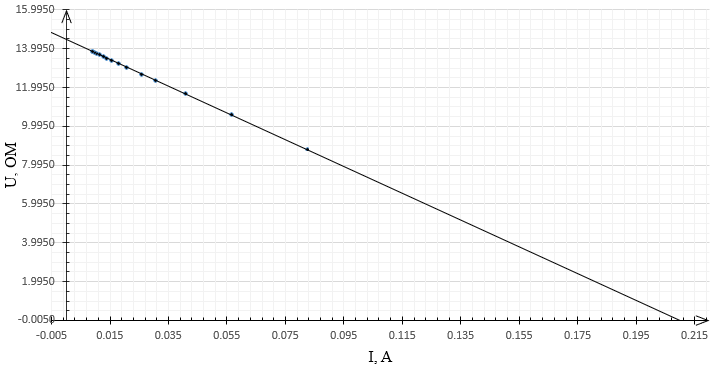
\includegraphics{graph1}
\end{center}
\item Рассчитаем внутреннее сопротивление источника $r = \frac{\varepsilon}{I_к} = \frac{14,49}{0,18} \approx 78,35$ и $I_m = \frac{\varepsilon}{2r} = \frac{14,49}{156,7} \approx 0,09$. 
\item Рассчитаем полезную мощность $P_1 = I^2R$, потери мощности $P_2 = I^2r$, полную мощность $P = I\varepsilon$ и КПД $\eta = 1 - I {I^{-1}}_к$ для каждого значения силы тока. Полученные данные представим в виде таблицы:
\begin{table}[h!]
\begin{center}
\begin{tabular}{|c|c|c|c|c|}
\hline
$I$, А & $P$, Вт & $P_1$, Вт &  $P_2$, Вт & $\eta$, \% \\
\hline
82,40 & 1,19 & 0,67 & 0,53 & 0,55\\
\hline
56,50 & 0,82 & 0,64 & 0,25 & 0,69\\
\hline
40,70 & 0,59 & 0,50 & 0,13 & 0,78\\
\hline
30,40 & 0,44 & 0,37 & 0,07 & 0,84\\
\hline
25,70 & 0,37 & 0,33 & 0,05 & 0,86\\
\hline
20,60 & 0,30 & 0,25 & 0,03 & 0,89\\
\hline
17,80 & 0,25 & 0,22 & 0,02 & 0,90\\
\hline
15,50 & 0,22 & 0,19 & 0,01 & 0,91\\
\hline
13,80 & 0,20 & 0,17 & 0,01 & 0,92\\
\hline
12,70 & 0,18 & 0,16 & 0,01 & 0,94\\
\hline
11,40 & 0,17 & 0,14 & 0,01 & 0,95\\
\hline
10,50 & 0,15 & 0,13 & 0,00 & 0,95\\
\hline
9,80 & 0,14 & 0,12 & 0,00 & 0,95\\
\hline
9,10 & 0,13 & 0,12 & 0,00 & 0,95\\
\hline
9,10 & 0,13 & 0,12 & 0,00 & 0,95\\
\hline
\end{tabular}
\end{center}
\end{table}
\item Построим график зависимости мощностей от силы тока:
\begin{center}
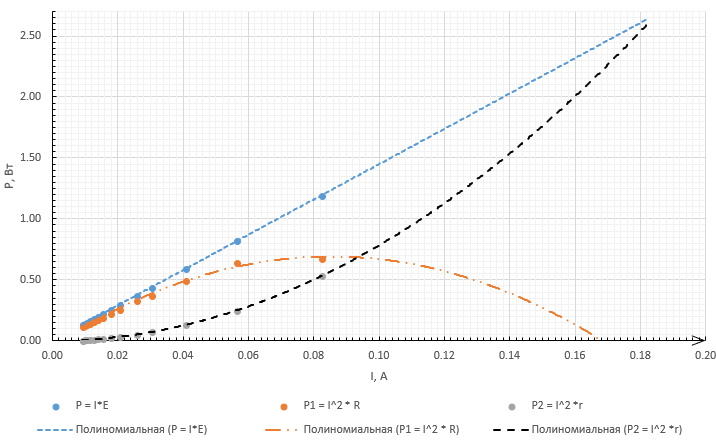
\includegraphics{graph2}
\end{center}
Полученные значения сходятся.
Построим график зависимости ЭДС от силы тока:
\begin{center}
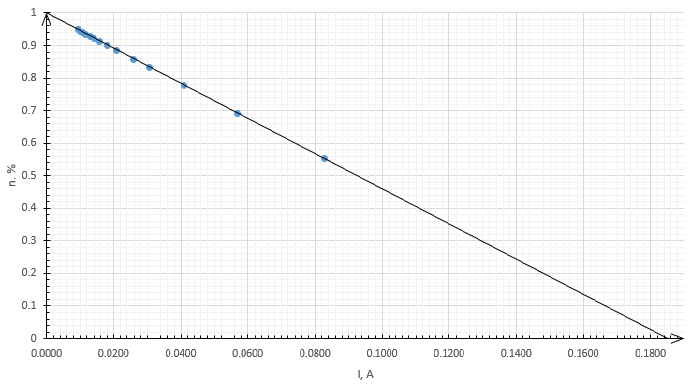
\includegraphics{graph3}
\end{center}
Полученные значения сходятся.
\section*{Вывод}
Экспериментальным путем был подтвержден закон Ома.

Помимо этого мы рассчитали силу тока короткого замыкания разными способами $I_{к1} \approx 0,18, I_{к2} \approx 0,19$ и $I_{к3} \approx 0,19$. Также рассчитали $I_{m1} \approx 0,09, I_{m2} \approx 0,10$ и  $I_{m3} \approx 0,10$.

Тот факт, что полученные значения достаточно близки, подтверждает правильность расчетов и рассуждений, на основе которых были произведены расчеты. 
 \end{enumerate}
\end{document}